\documentclass{article}
\usepackage{graphicx} 
\usepackage{subfiles}
\usepackage{natbib}
\usepackage{hyperref}
\setlength{\bibhang}{0.5in}
\bibliographystyle{apalike}
\usepackage{float}
%\usepackage{floatrow}
%  \floatsetup[table]{capposition=top}
\usepackage{booktabs}
\usepackage{tabularx}

\title{Tool Demo: Evaluating News Source Trustworthiness with NewsGuard for Misinformation Research}

\begin{document}
\maketitle

\section{Introduction}
Digital misinformation remains a major challenge, with research consistently highlighting the need for reliable, scalable tools to evaluate the trustworthiness of online news sources. 
NewsGuard is a popular tool in misinformation studies that rates news sources based on journalistic criteria. 
These ratings aim to help researchers identify untrustworthy information at the source level, especially valuable in tracking misinformation spread across digital platforms. 
This study evaluates the stability, completeness, and contextual applicability of NewsGuard’s ratings across multiple countries, contributing critical insights for researchers using NewsGuard in varied contexts.


\section{NewsGuard}
NewsGuard provides a robust trustworthiness score, derived from nine journalistic quality criteria that assess aspects such as misleading content, responsible information handling, and transparency about ownership. 
Each source receives a score on a 0-100 scale, with a threshold of 60 distinguishing trustworthy sources. 
The tool also offers additional context, such as political orientation and topic labels, adding further nuance to its ratings.

Since its inception in 2019, NewsGuard has grown to include a global selection of sources, initially focusing on U.S. media and later expanding to include sources from Europe, Canada, and Australia. 
The database regularly updates its ratings, ensuring coverage of new and evolving sources. 
Figure \ref{fig:trustworthiness_panel} visualizes this growth, illustrating the scale of additions over time and the stability of source ratings, particularly for U.S. outlets.


\begin{figure}[H]
    \centering
    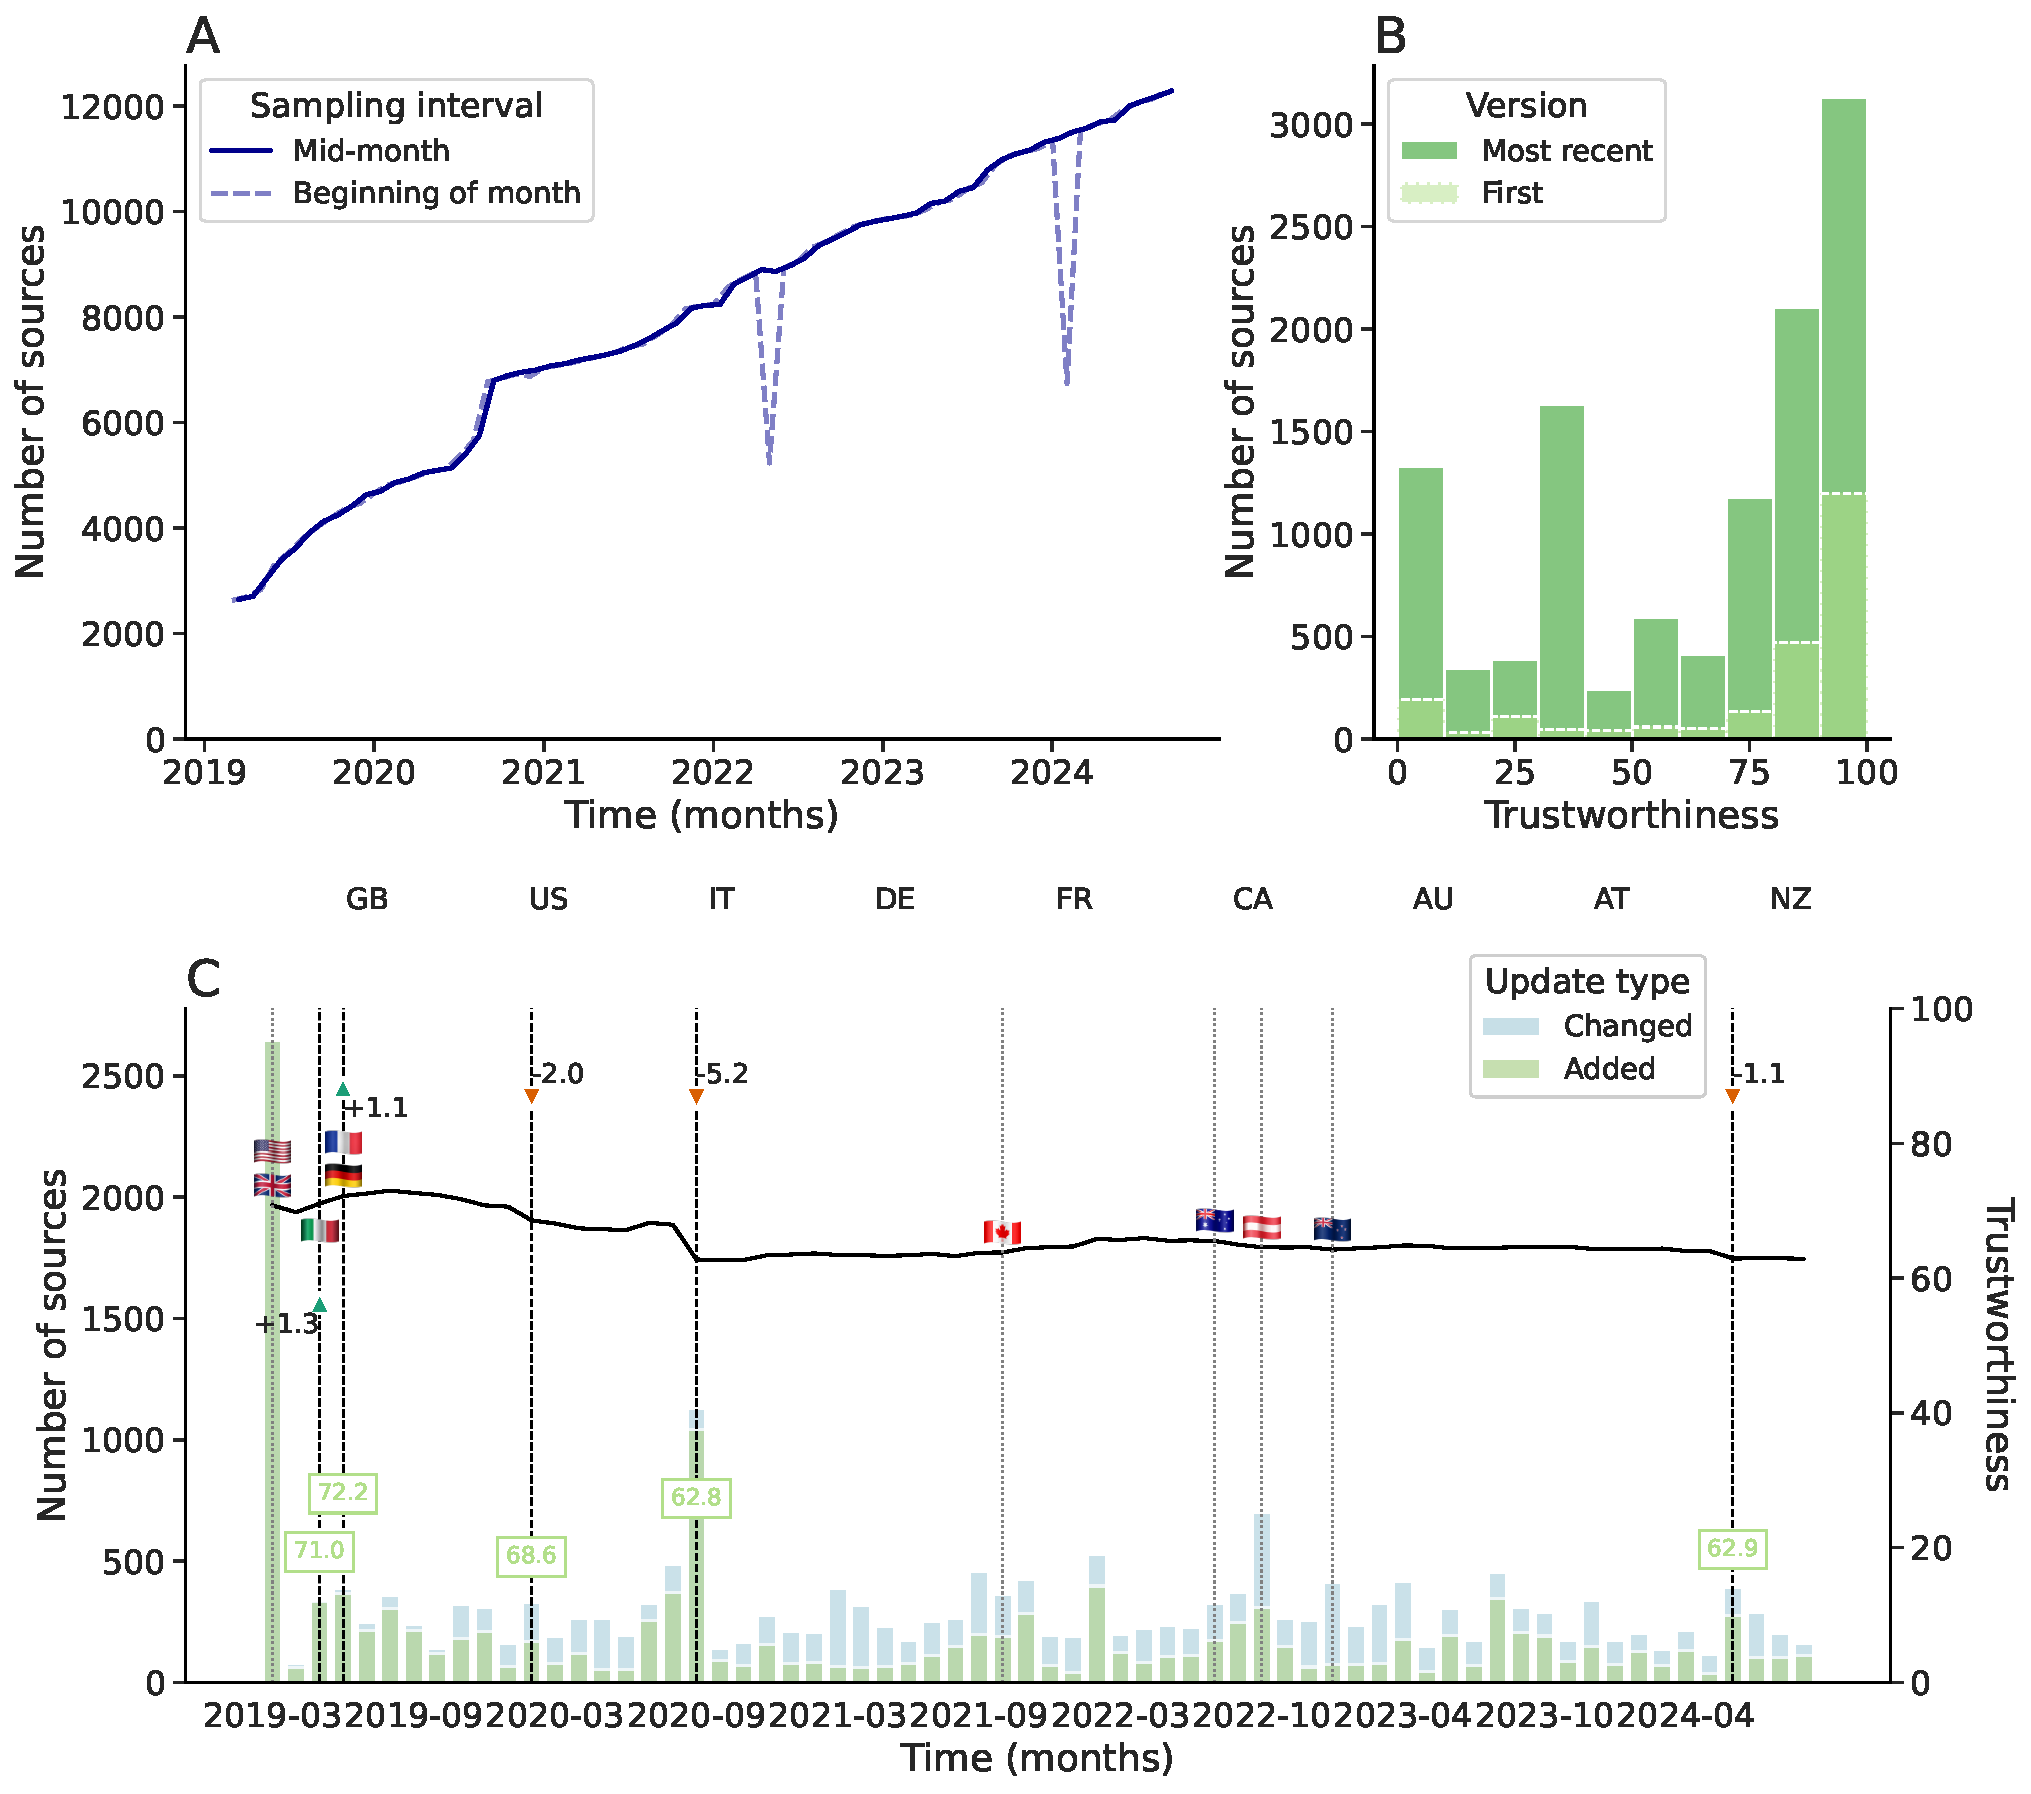
\includegraphics[width=\textwidth]{figures/trustworthiness_panel.pdf}
    \caption{Description of trustworthiness ratings with A showing the number of sources with rating over time based on two different sampling strategies: when sampling one snapshot of the database mid-month (solid line), we observe a steady increase, whereas sampling at the beginning of the month results in two irregular dips (dashed line). Panel B: distribution of trustworthiness in the first and most recent database as a histogram. Panel C: changes in trustworthiness scores over time (monthly granularity), with flags (respective country codes in order of appearance) and dotted lines indicating when countries were added and vertical lines highlighting the top five updates (i.e., major score changes, also shown with arrows). The height of the bars describes the number of sources added vs. changed, with colors indicating the proportions. Note: We include the average trustworthiness of sources added in green for the major changes. Countries are listed in the order added at the top of panel C.}
    \label{fig:trustworthiness_panel}
\end{figure}

\section{Methodology}
To assess NewsGuard's utility, we analyzed data spanning from 2019 to 2024, focusing on changes in source ratings, country-specific completeness, and comparisons with other source lists. 
The reproducibility of NewsGuard’s ratings over time was tested by examining variations across multiple database snapshots, particularly for U.S., U.K., and German sources. 
Plot 2 demonstrates the tool’s relative stability across snapshots, confirming consistency in major conclusions when using different versions of the database for established countries.



\begin{figure}[H]
    \centering
    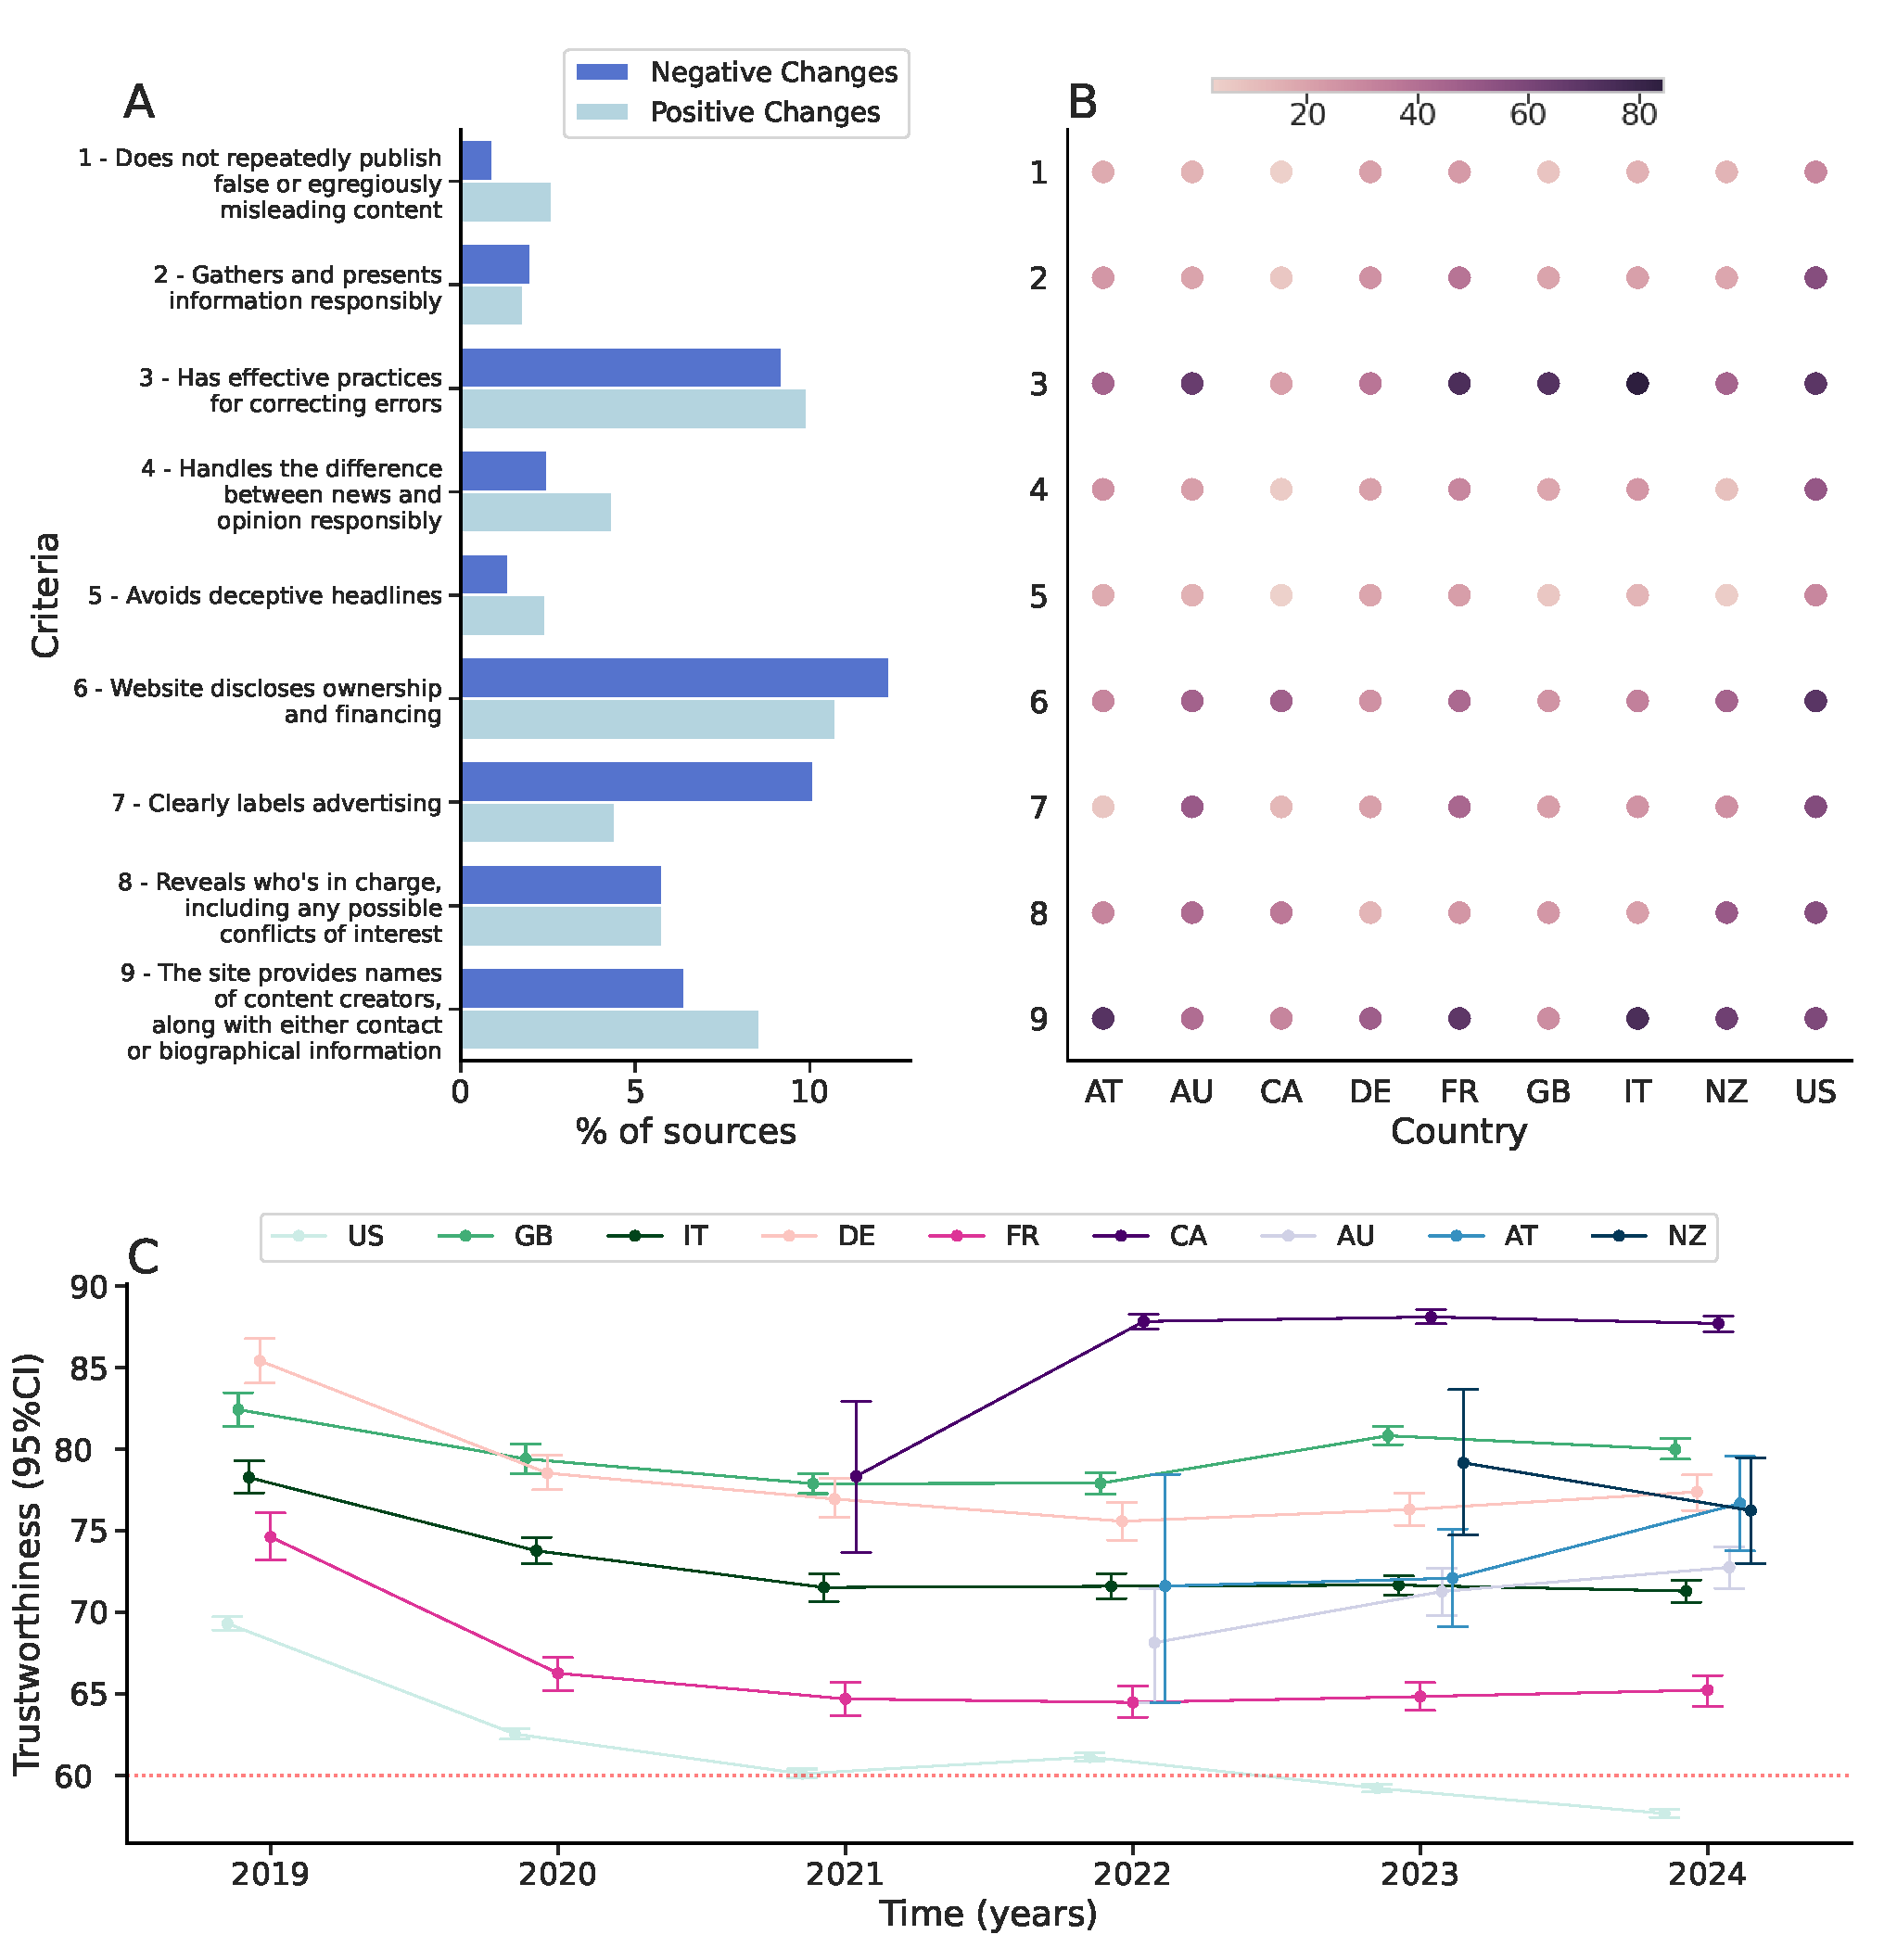
\includegraphics[width=\textwidth]{figures/criteria_panel_cropped.pdf}
    \caption{Panel A: percentage of sources that have stopped or started to fulfill a criterion, including multiple changes (positive vs. negative) of a single source. Panel B: percentage of sources that do not fulfill a criterion per country (July 15th, 2024). Panel C: trustworthiness per country over time (truncated to range from 55 to 90), aggregated per year with 95\% confidence intervals.}
    \label{fig:criteria_panel}
\end{figure}

\begin{figure}[H]
    \centering
    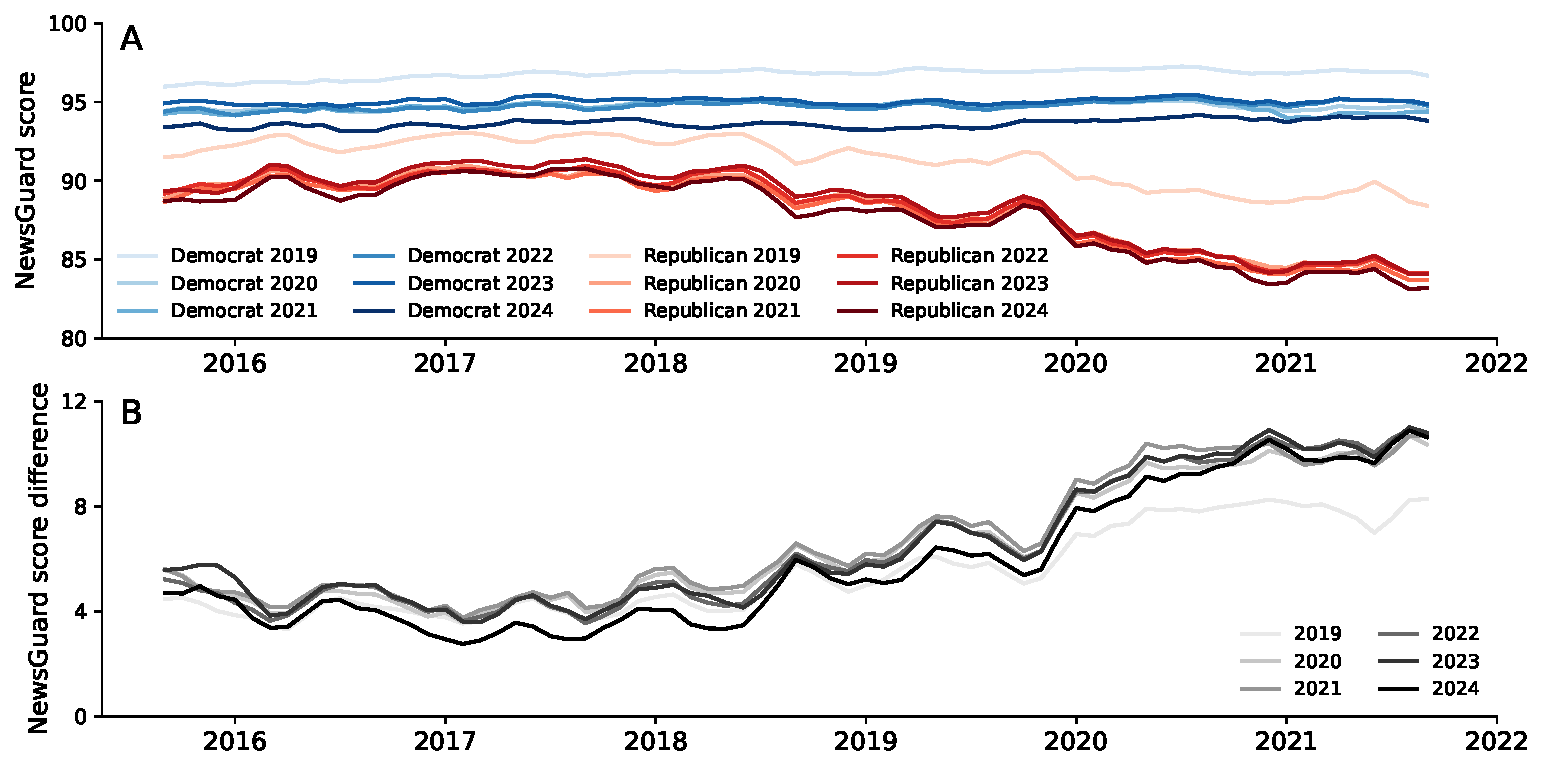
\includegraphics[width=\textwidth]{figures/politician_trustworthiness_replication_score_difference.pdf}
    \caption{Reproduction of the time series of NewsGuard scores of US Congress Members from Ref.~\cite{lasserSocialMediaSharing2022c} using different versions of the NewsGuard database from 2019 to 2024 (always taken from the first hour of March 1st of the given year). Panel A: average scores for Democrats and Republicans indicated in different shades of blue and red for each year. Panel B: difference between the average Democrat and average Republican score, indicated in different shades of grey for each year. The time series represent a moving average over three months.}
    \label{fig:reproduction}
\end{figure}

\section{Key Findings}
The analysis indicates that NewsGuard’s trustworthiness ratings have remained stable over time, with new entries generally maintaining similar scoring distributions (as shown in Plot 3). 
For well-established countries such as the U.S., U.K., and Germany, the reliability of the ratings is high, and coverage is near complete. 
However, for newer countries added more recently, such as New Zealand and Austria, coverage gaps may still affect accuracy.



Furthermore, NewsGuard’s topic and political orientation labels (illustrated in Plot 4) add valuable context for misinformation research. Sources rated as right-leaning tend to score lower on average, an observation consistent across countries. 
This highlights an essential characteristic of NewsGuard’s database: while comprehensive for mainstream topics and orientations, the tool may still exhibit limitations for niche or emerging outlets.

\begin{figure}[H]
    \centering
    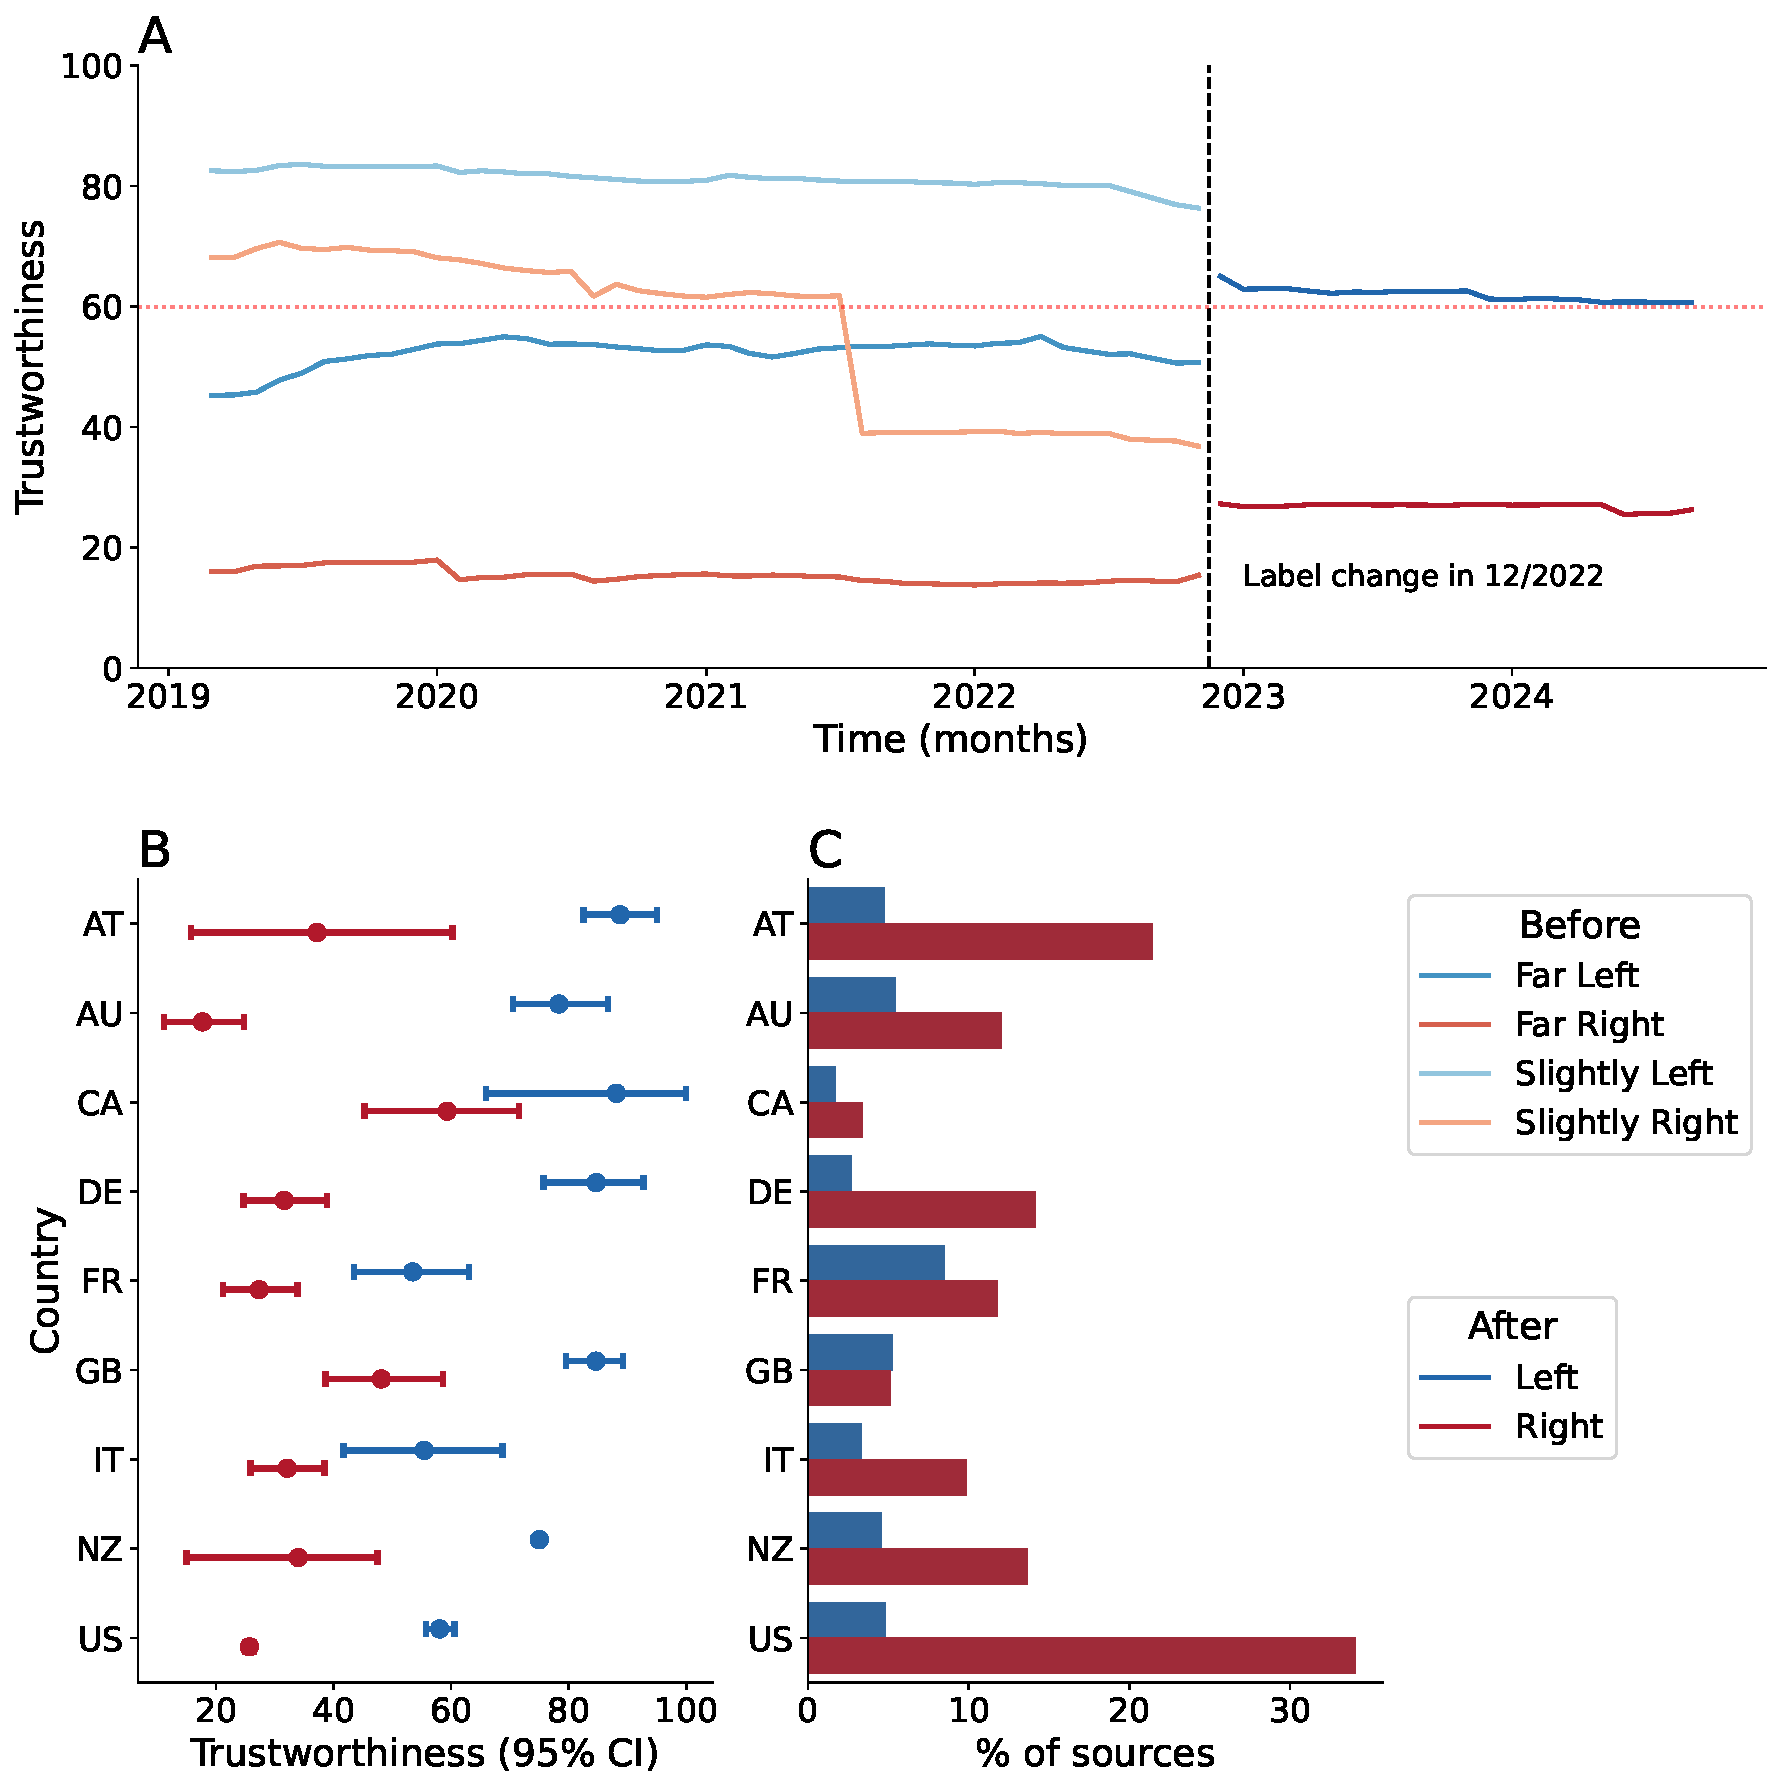
\includegraphics[width=\textwidth]{figures/orientation_panel.pdf}
    \caption{Trustworthiness averages by political orientation. Panel A: over time. Panel B: by country. Panel C: percentage of sources per country with political orientation, explaining differences in trustworthiness by country.}
    \label{fig:orientation_panel}
\end{figure}
\section{Recommendations}
The demonstration showcases how to navigate the NewsGuard interface, query source ratings, and interpret the accompanying contextual labels (e.g., political leanings and topic tags). 
The tool’s relevance lies in its stability and depth of data, making it highly useful for misinformation research across multiple contexts. 
Researchers can leverage NewsGuard not only for trustworthiness assessments but also to understand trends in topic-specific misinformation. 
For example, topics such as “political news” and “health misinformation” have shown significant variations in trustworthiness (see Plot 5), underlining the value of using NewsGuard’s combined topic and trustworthiness indicators.


\begin{figure}[!h]
    \centering
    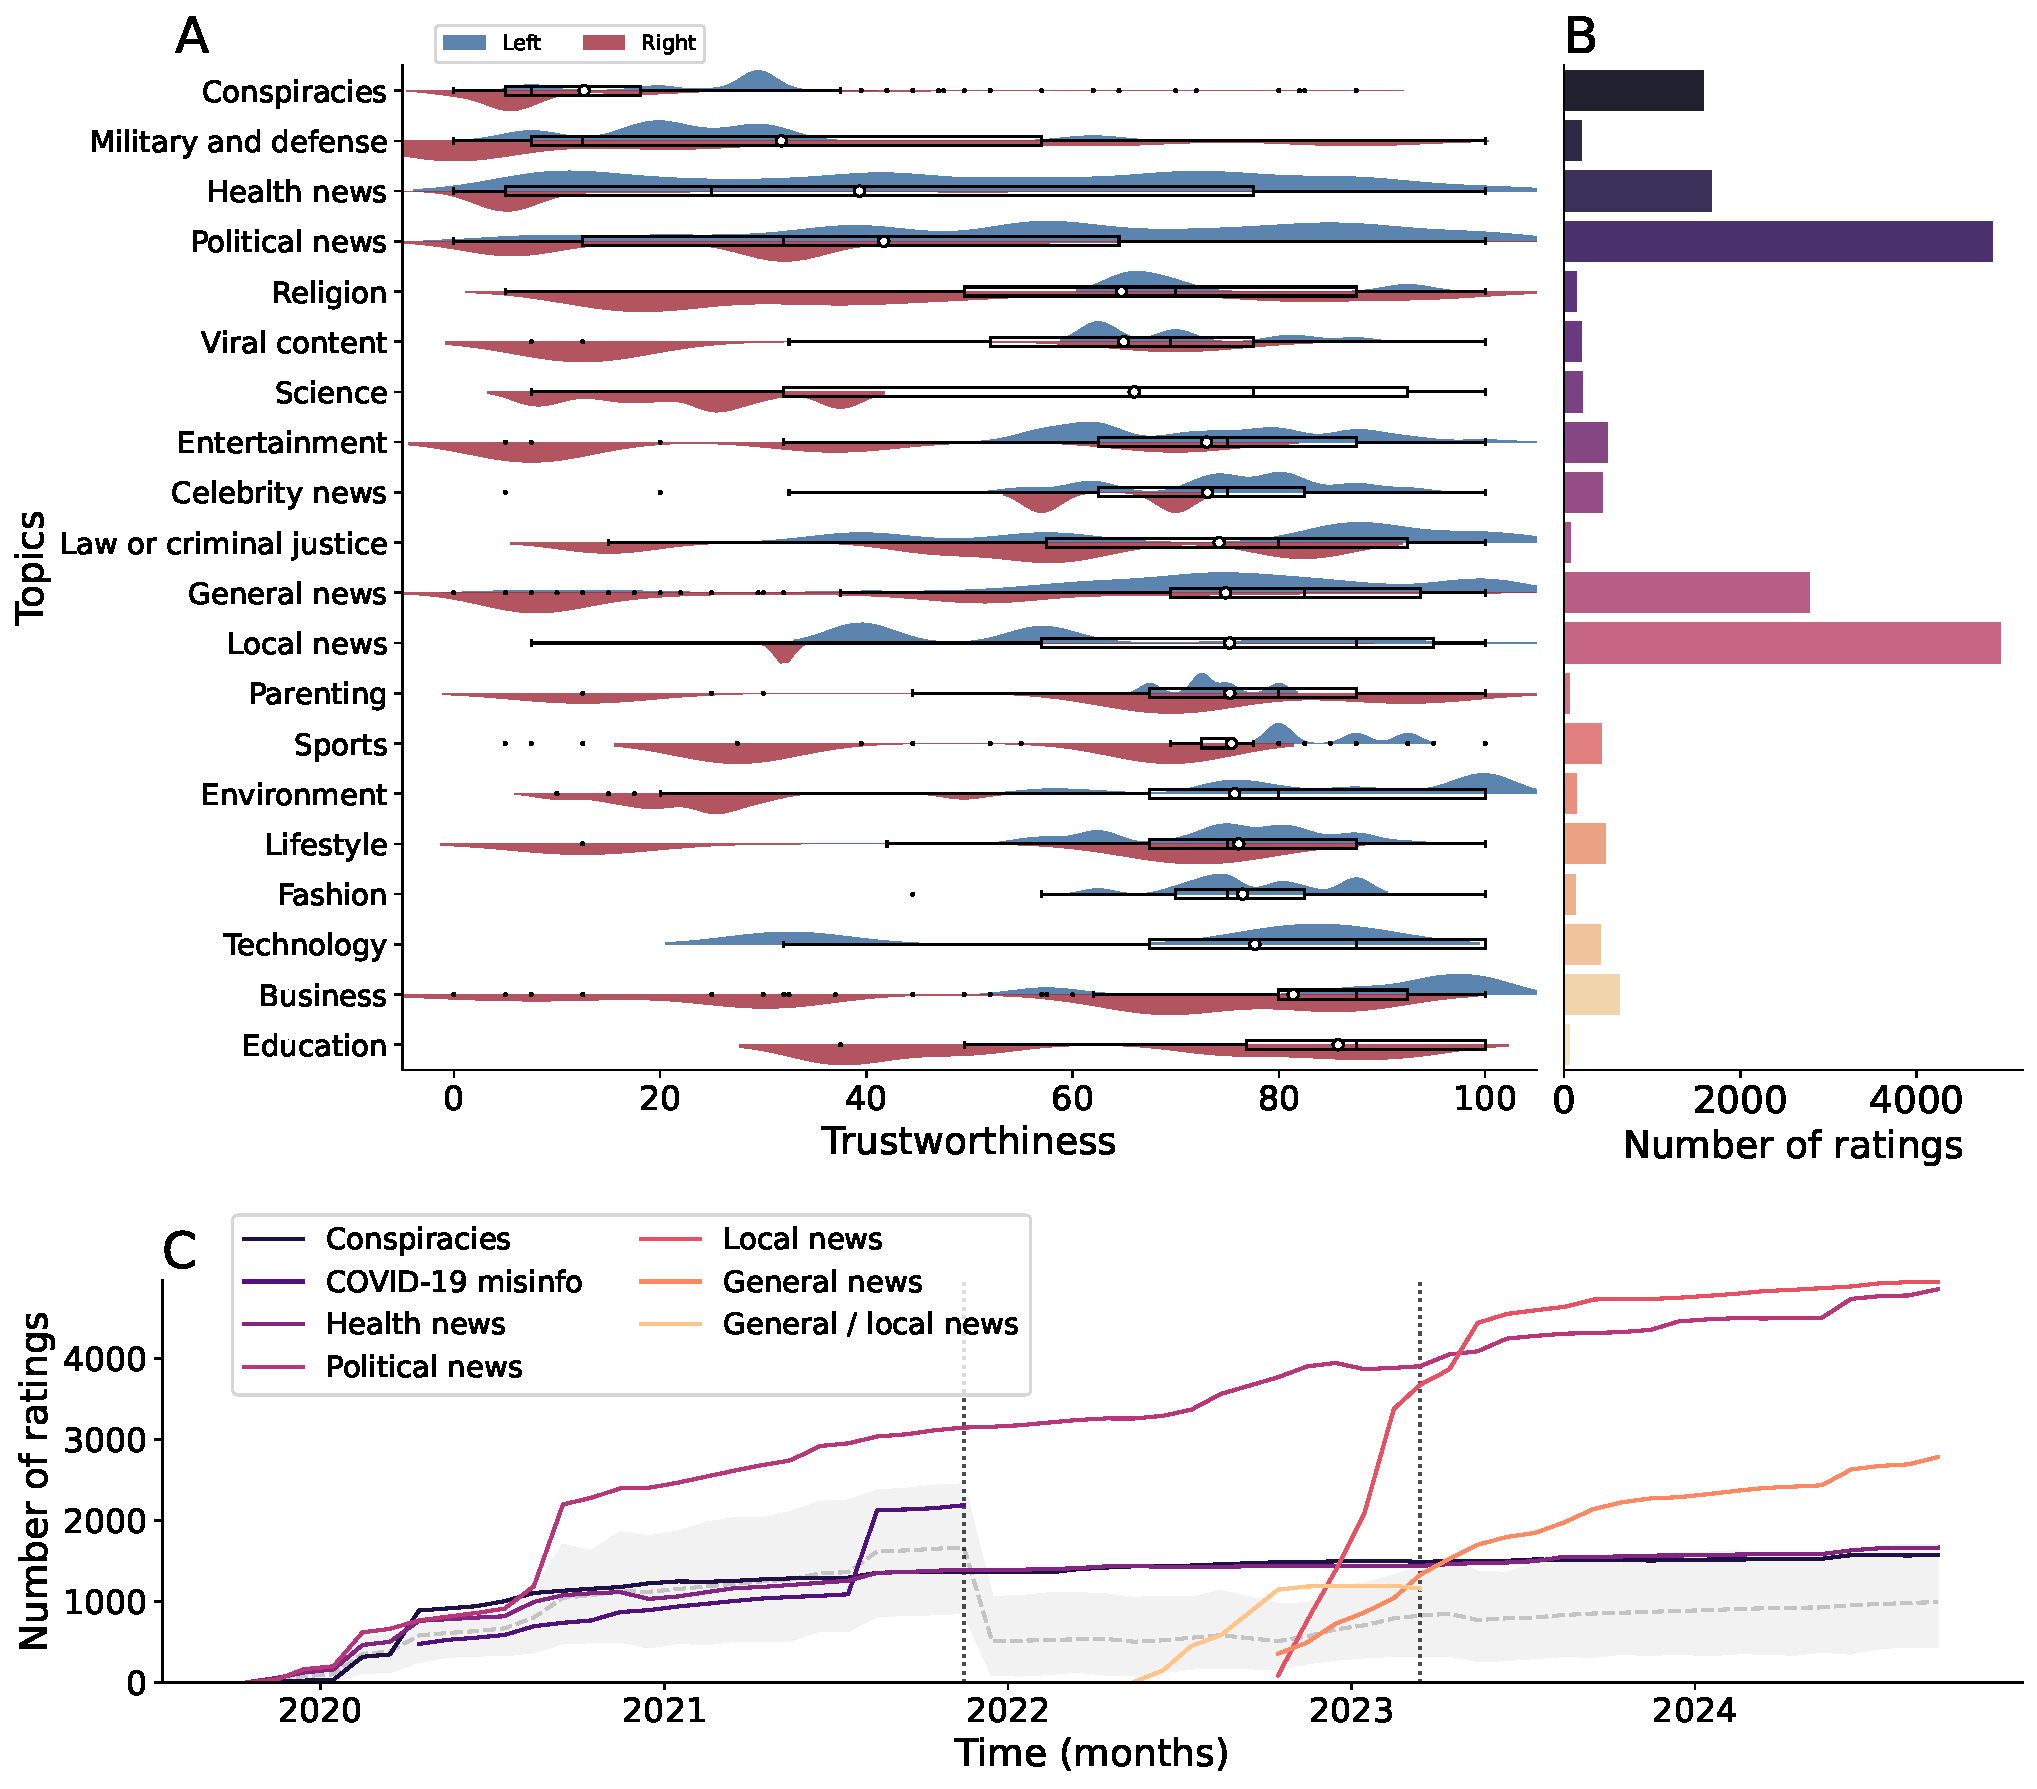
\includegraphics[width=\textwidth]{figures/topics_panel.pdf}
    \caption{A) shows the distributions of trustworthiness per topic and political orientation (left/right in blue/red, respectively), sorted by their average trustworthiness (white dot within the boxplot that represents the quartiles and whiskers show the whole range). 
    Note: We excluded topics with a count below 50. Some topics are abbreviated. B) gives the count of topics as of September 15th, 2024.
    C) shows the frequency of misinformation-related labels over time.
    Colored lines show the top five topics covered by untrustworthy sources. 
    The dotted, vertical lines show the removal of two of those labels.
    The grey and dashed line shows the average topic label count of those topics across all sources with the 95\%CI.}
    \label{fig:topics_panel}
\end{figure}

\section{Conclusion}
NewsGuard is a valuable asset for misinformation research, offering reliable, stable, and context-rich ratings of news sources. 
For researchers working on cross-national or time-sensitive misinformation studies, NewsGuard's data offers a trustworthy baseline, with the recommendation to ensure the most recent database version for countries added later. 
This study affirms NewsGuard’s utility in studying misinformation dynamics and provides researchers with a foundation for applying source-based approaches in diverse digital media landscapes.

\end{document}